\section{Deterministic Verifier and Epistemic Invariants}

A critical challenge in visual abstraction is solipsistic overfitting, where candidate search algorithms fit demonstrations via memorization rather than inferring generalizable rules. \texttt{NeuroARC.jl} implements an isolated verification harness:

\subsection{Verification Invariants}
Before any candidate is admitted into the verified execution pool, it must satisfy three deterministic gates:
\begin{enumerate}
  \item \textbf{Train Exact Reconstruction}: The candidate transformation must reconstruct 100\% of cells across all training demonstration output grids ($Y_i = f(X_i)$) with maximum cell residual equal to 0.0.
  \item \textbf{Informative Leave-One-Out (LOO) Evaluation}: Cross-validation across demonstration pairs is evaluated to detect parameter overfitting. When a rule contains free parameters, LOO folds are marked informative; parameter-free macros require verified cross-task firing to avoid single-task memorization.
  \item \textbf{Equivariance Gating}: Where task semantics exhibit geometric invariance, the candidate must commute with the dihedral group $D_8$ and background-preserving color permutations. If a candidate depends on directional or absolute spatial coordinates, equivariance is flagged as \texttt{untestable}, leading to an explicit \texttt{Incomplete} evaluation rather than a false positive certification.
\end{enumerate}

\subsection{Epistemic Limits of Verification}
The verifier certifies compliance with observed demonstration contracts and structural invariants; it does not and cannot certify ground-truth accuracy on held-out test grids. Post-run test evaluation is conducted strictly through isolated scoring harnesses against quarantined held-out labels after solver processes terminate.

\subsection{Molecular Track Recording as a Cross-Domain Verification Analogy}
Drukier et al.\ proposed using ordered nucleic-acid strands as a track-recording medium for energetic-particle interactions, with sequence-based readout used to reconstruct strand-break locations \cite{drukier2015new}. The design illustrates a general measurement principle: discriminating observations, spatial containment, and traceable readout can work together to separate candidate signals from backgrounds. Subsequent work by O'Hare et al.\ explored the detector concept through Monte Carlo simulations while identifying unresolved experimental challenges \cite{ohare2022particle}.

The connection to \texttt{NeuroARC.jl} is methodological rather than physical or mathematical equivalence. Directional discrimination motivates controlled tests of orientation-sensitive behavior; layered containment motivates explicit isolation and acceptance invariants; and molecular barcoding motivates reproducible candidate provenance. These analogies generate testable software-design hypotheses, but do not establish \texttt{NeuroARC.jl}'s equivariance properties, improve its sample complexity, validate its quarantine mechanism, or provide evidence for radiation-driven prebiotic chemistry. Each claim requires independent evidence under its own model and evaluation protocol.

\begin{figure}[htbp]
  \centering
  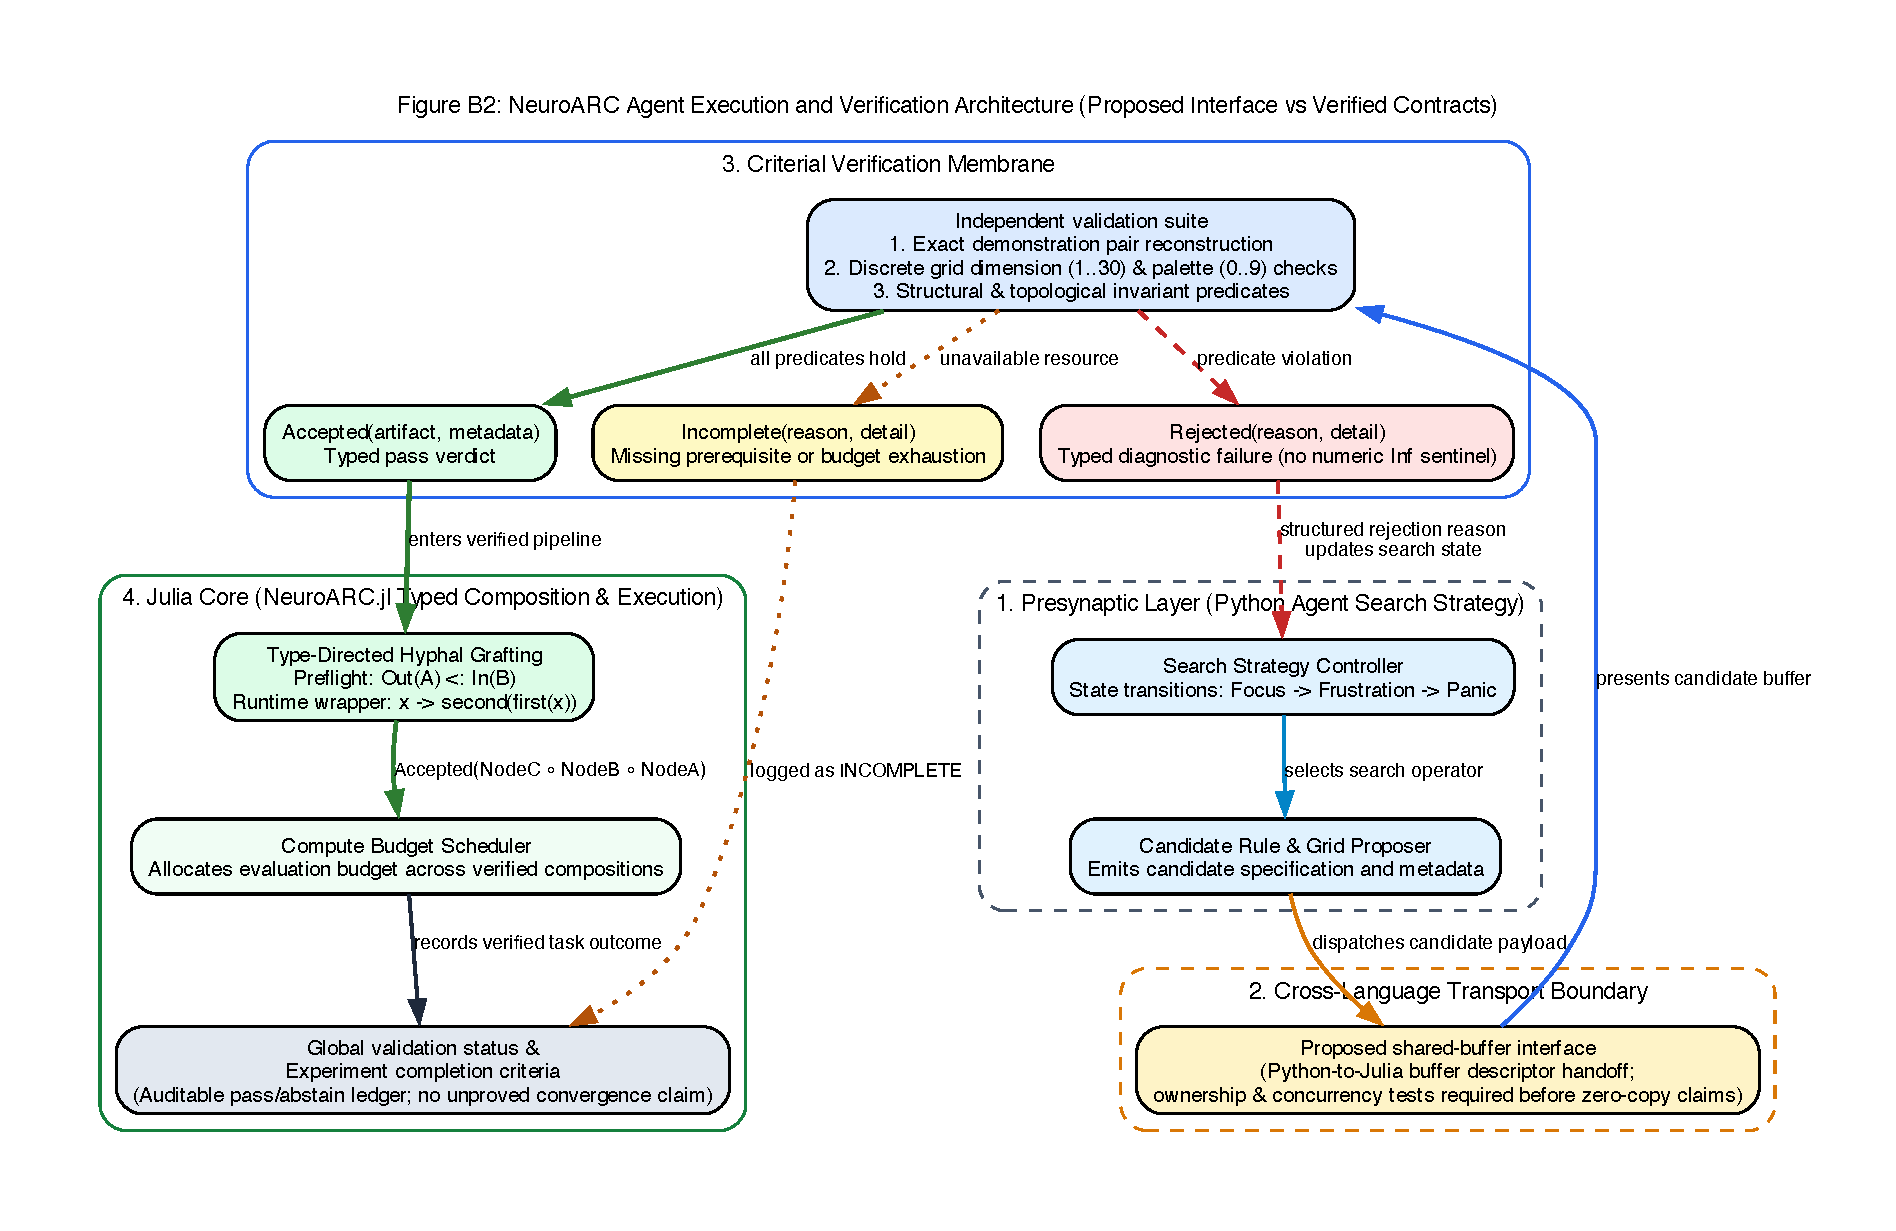
\includegraphics[width=\textwidth]{figures/figure_b2_agent_execution.pdf}
  \caption{\textbf{Figure B2: NeuroARC Agent Execution and Verification Architecture.} Depicts the separation between presynaptic heuristic search, cross-language transport buffers, the criterial verification membrane, and the verified Julia composition core.}
  \label{fig:agent_execution}
\end{figure}
